\documentclass[12pt]{article}
\usepackage[utf8]{inputenc}
\usepackage{graphicx} 
\usepackage{wrapfig}
\usepackage[dvipsnames]{xcolor}
\usepackage{moreverb}
\usepackage{ragged2e}
\renewcommand\refname{Referencias}
\title{Elementos de la programación Python 1.}
\author{\textcolor{JungleGreen}{Olga María Fimbres Morales}}
\date{17 de Enero 2016}
\begin{document}
\begin{titlepage}

\begin{center}
\begin{large}
Universidad del Estado de Sonora\\
\end{large}
\vspace*{0.15in}
División de Ciencias Exactas y Naturales.\\
\vspace*{0.15in}
Licenciatura en Física. \\
\vspace*{0.6in}
\begin{large}
Física Computacional 1\\
\end{large}
\vspace*{0.2in}
\begin{Large}
\textbf{{\textcolor{Red}{El Espacio Fase.}}} \\
\end{Large}

%\begin{Large}
%\textbf{{\textcolor{Red}{Péndulo.}}} \\
%end{Large}
%\vspace*{-1in}

\rule{80mm}{0.1mm}\\
\vspace*{0.1in}
\begin{large}
{\textcolor{JungleGreen}{Olga María Fimbres Morales}}\\
17 de Marzo de 2016\\
\end{large}
\end{center}
\end{titlepage}

\pagebreak
\section*{Introducción.}
 Nuevamente abordamos el modelo físico de péndulo, pero esta vez de una forma distinta a la que se ha venido haciendo, ya que durante el desarrollo de esta práctica lo que se busco lograr fue el generar un espacio fase de múltiples soluciones para el modelo que ya se tenia, otra vez, el péndulo.\\
 
 Sabemos, que una ecuación diferencial posee lo que se llama una familia de soluciones que se generan a partir de aquellas mas elementales que surgen a partir de encontrar una solución general al problema, a esto, a esta familia de soluciones es a lo que nos referimos con espacio fase.\\
 
 En el desarrollo de esta actividad, se generaron a aquellas posibles soluciones a partir de ciertas condiciones iniciales, dígase ángulo y velocidad angular inicial, durante un periodo de tiempo, permitiéndonos de esta forma observar la forma en que se comportaría el péndulo teniendo distintas condiciones iniciales.
 
 
\section*{\textcolor{Red}{Espacio Fase.}}
El espacio pase es una representación geométrica de las trayectorias de una sistema dinámico en el plano fase. Cada grupo de condiciones iniciales representa una curva o punto diferente en el.\\

Son sumamente útiles al momento de estudiar sistemas dinámicos, consisten en un gráfico de las trayectorias en el espacio; nos permiten conocer diferente información como la velocidad que lleva en un determinado momento, el desplazamiento o los límites entre los cuales se desarrolla el sistema.\\

 Utilizan diferente simbología por ejemplo, la trayectoria se representa con flechas, los puntos estables con puntos y los puntos inestables con círculos.\\
	

Existen diferentes ejemplo de donde podemos utilizar los espacios fases, algunos de ellos son:
\begin{itemize}
\item Péndulo simple.
\item Oscilador armónico simple.
\item Oscilador de Van der Pol.
\item Diagrama de bifurcación.
\item Plano de parámetro.
\end{itemize}

\begin{center}
      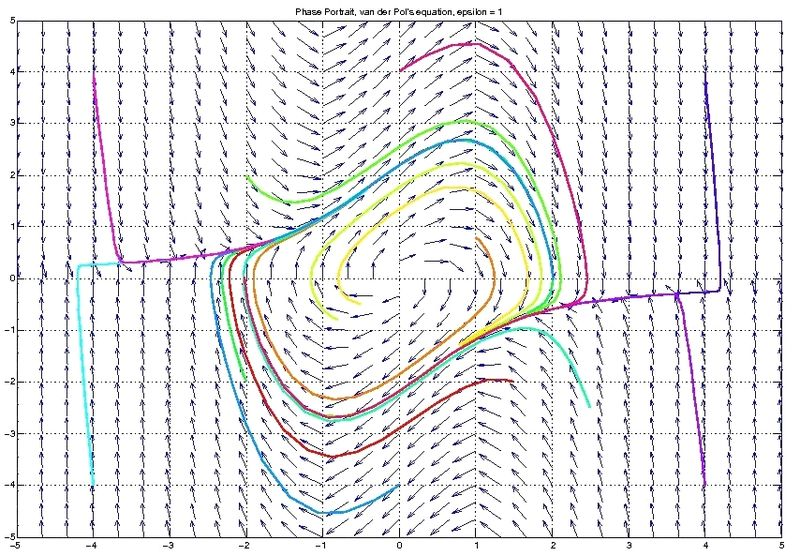
\includegraphics[scale=0.4]{espaciofase.jpg}
      
      \caption{Espacio fase del oscilador de Van der Pol \cite{Img1}.}
    \end{center}

Como podemos ver, son una herramienta que nos permite conocer el estado del modelos que estemos estudiando, por lo que para ciertas condiciones iniciales nos es posible saber que trayectoria seguirá, que velocidad tendrá y como se comportara a lo largo del tiempo.


\pagebreak
\section*{\textcolor{LimeGreen}{Problema.}}
El desarrollo de esta actividad consistió en realizar la gráfica de un espacio fase de las soluciones del péndulo simple a partir de un programa para el espacio fase del crecimiento de las poblaciones de zorros y conejos, el cual se encontraba disponible en la biblioteca de SciPy Cookbook\cite{5}.\\

Nuevamente se utilizó la herramienta $odeint$ utilizada en la práctica número 5 para realizar la integración de nuestra funciones y de esta forma encontrar las diferentes soluciones a partir de distintas condiciones iniciales.\\

Primeramente fue necesario comprender la forma en que el código que se nos proporcionó trabajaba y la forma en que graficaba los resultados obtenidos de las integraciones de las funciones  para crear el siguiente espacio fase:

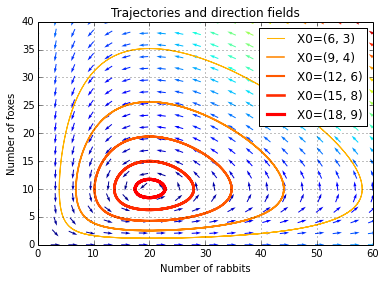
\includegraphics{espacioconejos.png}

Que como podemos observar nos muestra la forma en que se comporta el número de conejos y zorros vivos en una cierta área en distintas condiciones iniciales, donde los conejos corresponden al eje X y los zorros al eje Y.\\

Apoyándonos en actividades pasadas donde ya habíamos desarrollado la integración de la ecuación diferencial del péndulo simple solamente fue necesario tomar como referencia el ámbito que crea la gráfica del espacio fase del código que se nos proporcionó y utilizando condiciones iniciales adecuadas para crear el espacio fase deseado fue que se logro crear un diagrama adecuado. Generando de esta forma el siguiente código:\\

\begin{boxedverbatim}
import numpy as np
import matplotlib.pyplot as plt
from scipy.integrate import odeint
import pylab as p
from scipy import integrate

b = 0.0 #fricción
g = 9.8 #gravedad
l = 1. #longitud de la cuerda
c = g/l

#condiciones iniciales 
X_f0 = array([ -4*np.pi , 4*np.pi])
X_f1 = array([ -2*np.pi, np.pi*0])
t = np.linspace(0, 20, 300) #rango de tiempo

def pend(y, t, b, c):
     theta, omega = y
     dydt = [omega, -b*omega - c*np.sin(theta)]
     return dydt

values  = linspace(-1, 1, 60)                          
# position of X0 between X_f0 and X_f1
vcolors = p.cm.terrain_r(linspace(0.5, 1., len(values)))  
# colors for each trajectory
vcolors2 = p.cm.winter_r(linspace(0.5, 1., len(values)))
f2 = p.figure()
\end{boxedverbatim}
\\
\begin{boxedverbatim}
#-------------------------------------------------------
# plot trajectories
for v, col in zip(values, vcolors):
    X0 = v * X_f0                               
    # starting point
    X = integrate.odeint( pend, X0, t, (b, c) )        
    p.plot( X[:,0], X[:,1], lw=3.5*v, color=col,
    label='X0=(%.f, %.f)' % ( X0[0], X0[1]) )
     
for v, col in zip(values, vcolors):
    X0 = v * X_f1                               
    # starting point
    X = integrate.odeint( pend, X0, t, (b, c) )        
    p.plot( X[:,0], X[:,1], lw=3.5*v, color=col,
    label='X0=(%.f, %.f)' % ( X0[0], X0[1]) )

#-------------------------------------------------------
p.title('Espacio fase del pendulo simple.')
p.grid()
p.xlim((-4*np.pi)/2, (4*np.pi)/2)
p.ylim(-4*np.pi, 4*np.pi)
f2.savefig('rabbits_and_foxes_2.png')
\end{boxedverbatim}
\\
Podemos observar que comenzamos por especificar todas aquellas herramientas que utilizaremos durante el desarrollo del programa, todas ellas previamente utilizadas.\\

Continuamos especificando las constantes para nuestro sistema del péndulo simple, como siempre la fricción sera nula, la gravedad la constante terrestre y la longitud de la cuerda un metro. Ahora, las condiciones iniciales de nuestro sistema serán en dos distintas direcciones, f1 correspondiente al ángulo inicial y f2 correspondiente a la velocidad angular inicial, además de la variante del tiempo; las primeras dos las construimos como arreglos entre dos diferentes posiciones dependientes de $\pi$ y el último como una secuencia de 300 números igualmente espaciados entre 0 y 20.\\

Ahora, procedemos a especificar la función con la que vamos a trabajar, que como recordara, es la misma utilizada en actividades anteriores. Después, definimos la posición inicial, el cual resulta una sucesión de números entre -1 y 1, y los colores que se utilizaran para graficar; Python cuenta con una amplia gama de colores solidos y degradados para realizar las gráficas, por lo que esto resulta decisión del programador.\\

Pasamos ahora a realizar graficar las trayectorias, pero primero resulta necesario generar los datos a graficar; lo cual se logra con un ciclo que toma los arreglos que especificamos como condiciones iniciales. Ahora, pasamos a realizar la integración de la ecuación del péndulo simple junto con todos aquellos parámetros que le conciernen, que como ya sabemos logramos con la herramienta $odeint$.\\

Esto debe realizarse dos veces, una con nuestras condiciones f1 y otra con las condiciones f2 para que de esta forma seamos capaces de cubrir un mayor número de casos para el péndulo.\\

Finalmente, graficamos los arreglos formados por la integración de forma que una columna sera las ordenadas y la otra las abscisas.







\pagebreak

\section*{\textcolor{RoyalBlue}{Resultados}}
Una vez que logramos que nuestro código funcionara de la manera adecuada, para lo cual puede resultar necesario jugar un poco con los límites utilizados en las condiciones iniciales y el punto inicial, obtenemos el espacio fase que nos muestra las posibles soluciones para la ecuación diferencial del péndulo simple:

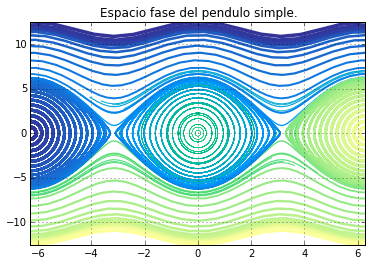
\includegraphics{actividad7.png}

Utilizando esto como apoyo podemos conocer la posición y la velocidad angular que poseerá en diferentes momentos y para distintas condiciones iniciales, así como conocer sus puntos de equilibrio, por ejemplo, a simple vista podemos observar que uno de sus puntos de equilibrio es el punto (0,0) lo cual nos dice que para un ángulo inicial cero y una velocidad angular cero el péndulo no se moverá.\\

De igual modo podemos seleccionar un punto cualquiera, dentro de los límites de nuestro diagrama de fase, formando sus coordenadas por ángulo y velocidad angular inicial y conocer el comportamiento que el péndulo tendrá para dichas condiciones iniciales.



\section*{\textcolor{Purple}{Anexos}}
\subsection*{\textcolor{RubineRed}{Código Zorros y Conejos}}
\begin{boxedverbatim}
from scipy import integrate
import numpy as np
import matplotlib.pyplot as plt

l = 1. #longitud de la cuerda
g = 9.81

#periodo para oscilaciones pequeñas
To = 2*np.pi*sqrt(l/g) 

#periodo para oscilaciones arbitrarias
#definir la función a integrar

#theta_0 = np.linspace(0, np.pi-0.001 ,100)

X = lambda theta: 1.0/(np.sqrt(np.cos(theta)-np.cos(theta_0)))
#ciclo para integrar
theta_0 = 0.0
while (theta_0 < np.pi-0.08): 
#es necesario restringirlo a un numero antes de pi, 
pero si este es muy pequeño 
el programa tiene problemas para correr
    theta_0 = theta_0 + 0.05
    int2 = integrate.quad(X, 0.0, theta_0)    
    
    #print(int2[0])
    #theta = (theta_0*360)/np.pi
    #print(theta)
    T = 4*sqrt(l/(2*g))*int2[0]
    #print(T)
    Z = T/To
    #print(Z)
    #print(theta_0)
    plt.plot(theta_0 ,Z,'o', label='Error relativo')
    plt.grid(True)
    plt.xlabel('Theta',fontsize=15)
    plt.ylabel('T/To',fontsize=15)
    v=[0,np.pi/2,1,1.2]
    axis(v)
    #plt.legend()
    #plt.show()
\end{boxedverbatim}

\subsection*{\textcolor{RubineRed}{Espacio fase Zorros y Conejos.}}
\begin{boxedverbatim}
values  = linspace(0.3, 0.9, 5)                          
# position of X0 between X_f0 and X_f1
vcolors = p.cm.autumn_r(linspace(0.3, 1., len(values)))  
# colors for each trajectory

f2 = p.figure()

#-------------------------------------------------------
# plot trajectories
for v, col in zip(values, vcolors):
    X0 = v * X_f1                               
    # starting point
    X = integrate.odeint( dX_dt, X0, t)         
    # we don't need infodict here
    p.plot( X[:,0], X[:,1], lw=3.5*v, color=col,
     label='X0=(%.f, %.f)' % ( X0[0], X0[1]) )

#-------------------------------------------------------
# define a grid and compute direction at each point
ymax = p.ylim(ymin=0)[1]                        
# get axis limits
xmax = p.xlim(xmin=0)[1]
nb_points   = 20

x = linspace(0, xmax, nb_points)
y = linspace(0, ymax, nb_points)

X1 , Y1  = meshgrid(x, y)                       
# create a grid
DX1, DY1 = dX_dt([X1, Y1])                      
# compute growth rate on the gridt
M = (hypot(DX1, DY1))                           
# Norm of the growth rate
M[ M == 0] = 1.                                
# Avoid zero division errors
DX1 /= M                                        
# Normalize each arrows
DY1 /= M
\end{boxedverbatim}
\pagebreak

Continuamos con el código.\\

\begin{boxedverbatim}
#-------------------------------------------------------
# Drow direction fields, using matplotlib 's quiver function
# I choose to plot normalized arrows 
and to use colors to give information on
# the growth speed
p.title('Trajectories and direction fields')
Q = p.quiver(X1, Y1, DX1, DY1, M, pivot='mid', cmap=p.cm.jet)
p.xlabel('Number of rabbits')
p.ylabel('Number of foxes')
p.legend()
p.grid()
p.xlim(0, xmax)
p.ylim(0, ymax)
f2.savefig('rabbits_and_foxes_2.png')
\end{boxedverbatim}
\pagebreak
\begin{thebibliography}{X}
 \bibitem{1} \textsc{Wikipedia, The free encyclopedia; "Phase portait"; 2016}{content...}
 \bibitem{Img1} \textsc{By Ashraful; via Wikimedia Commons;"Phase portrait"}
 \bibitem{5} \textsc{SciPy Cookbook; Matplotlib: Lotka volterra tutorial.}
\end{thebibliography}
\end{document}